% \chapter[基于WordNet构建的知识关联网络驱动的语义关联度计算]{\texorpdfstring{基于WordNet构建的知识关联网络驱动 \protect\\ 的语义关联度计算}{基于WordNet构建的知识关联网络驱动的语义关联度计算}}
\chapter{基于WordNet的语义关联度模型}
\label{chap:chap03}
本章采用WordNet作为构建知识关联网络的知识库,并采用更具表达能力的分布式向量来表征实体语义信息,由此利用WordNet中实体的语义信息来丰富词语间的语义关联度度量。

\section{WordNet简介}

WordNet作为一种英文词法关系库,其按照单词(主要包含名词、动词、形容词和副词)之间的语义内容和词法关系,由专家与计算机合作将大量英文单词划分为一组组同义词集。这种按照意义分组的创建方式使得WordNet即不局限于传统词法词典,也不同于同义词词林,WordNet不仅仅是用同义词集的方式去展示客观概念或主观事物,同义词集之间更由不同语义关系相关联着,这些关系有上下位关系(hyponymy)、整体部分关系(meronymy)、继承关系(entailment)等。如图\ref{chap3-1}所示,对于单词\emph{apple},WordNet中有两个实体与之对应,这两个实体分别描述了\emph{apple}作为一种水果的意义和作为一种植物的意义,同时这两个实体又分别有自己的关系属性,连接了其他与之关联的实体。

%选用WordNet的理由
\begin{figure}[!ht]
    \centerline{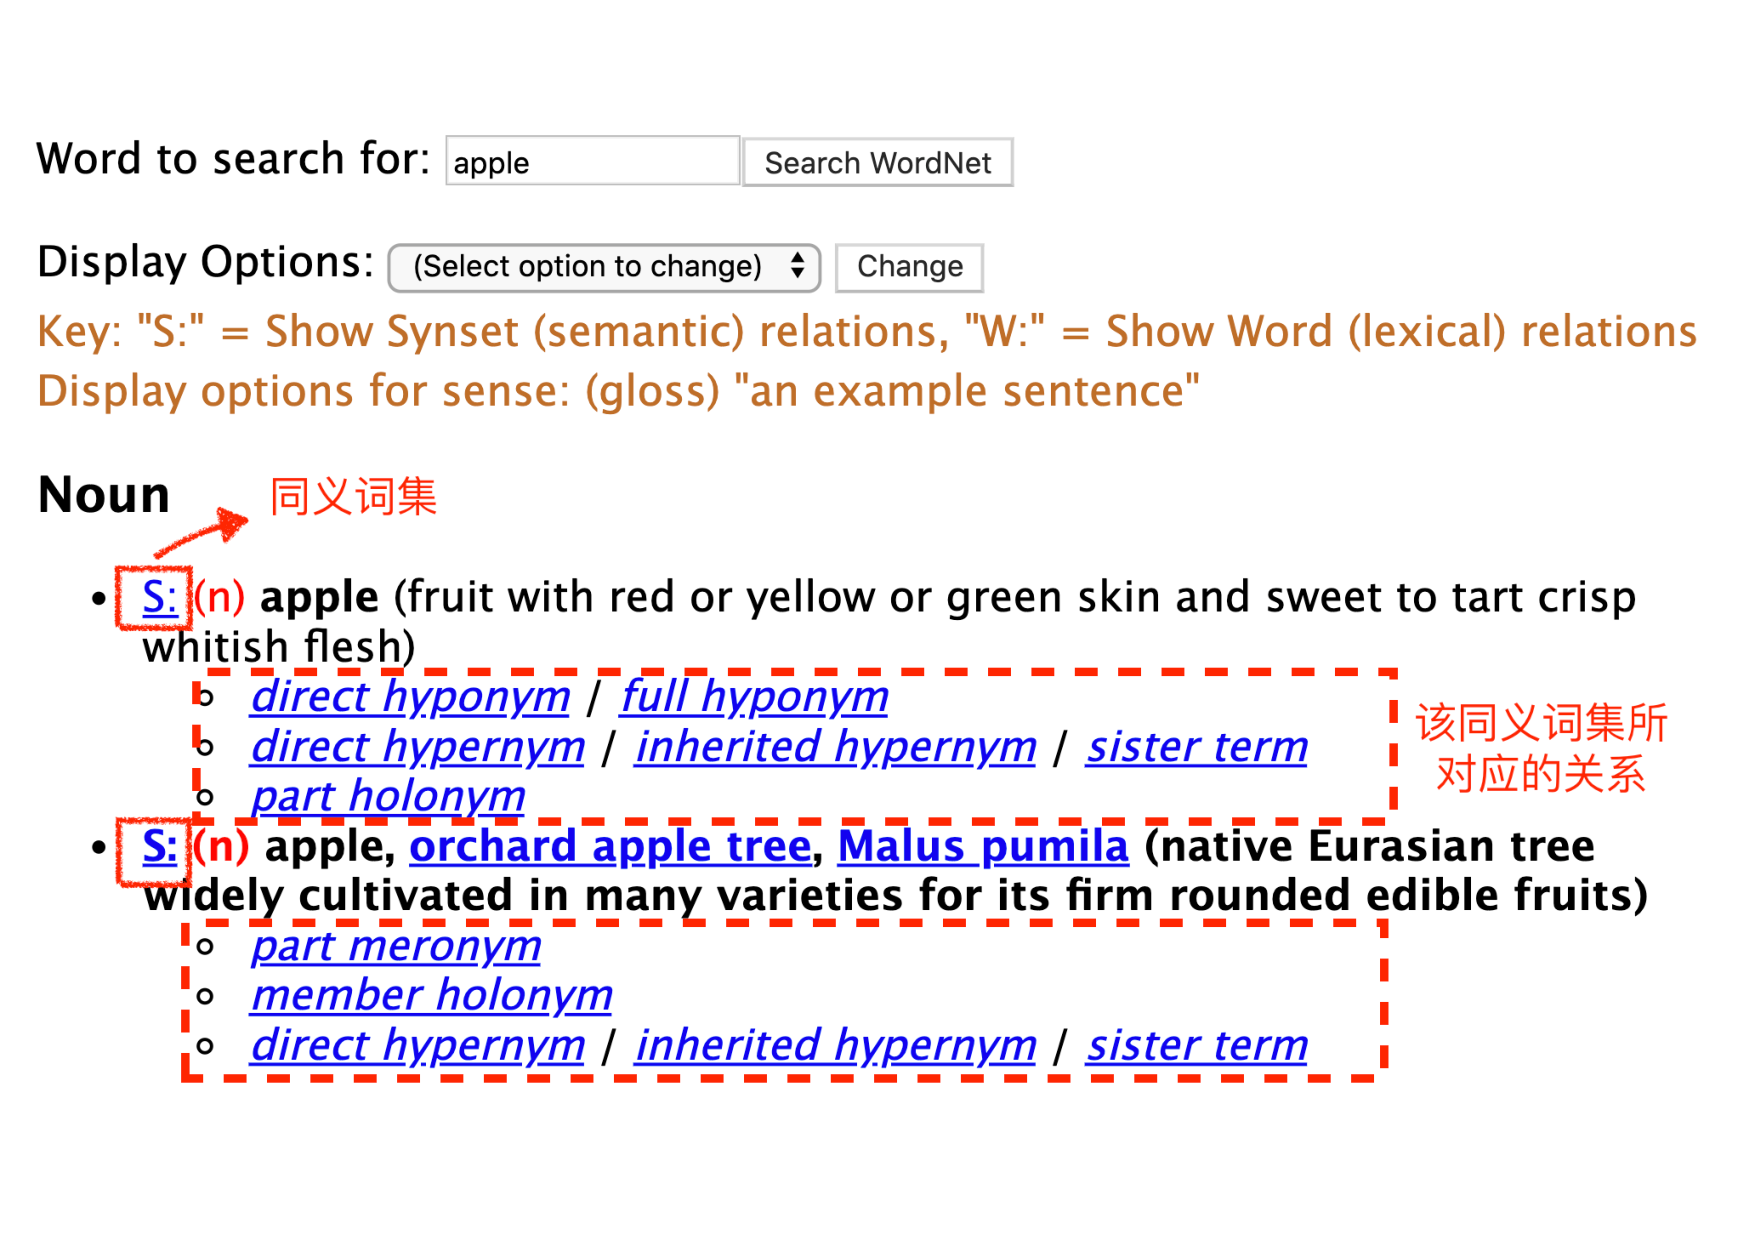
\includegraphics[width=0.8\textwidth]{chap3-1.pdf}}
    \smallcaption{WordNet同义词集示例}
    \label{chap3-1}
\end{figure}

传统研究者\cite{its/Rada89, Leacock98, wu1994verb, tkde/LiBM03}主要利用WordNet中同义词集的距离信息来衡量词语之间的语义差别,这种方法多用来建模词语间的层次关系,在语义相似度方面表现较好,但是对于涉及多种语义关系的关联度度量,这种方法表现不太好。为了弥补这些缺点,本文通过网络嵌入的方式学习到更具表达能力的分布式向量表示,由此来更好的完成语义关联度度量。

%构建
\section{知识关联网络构建}
对于知识关联网络的构建,首先要解决的问题是建立起词语与实体之间的直接联系。幸运的是,WordNet中提供了相应的查询接口来得到与词语相关的实体,其中最常用的接口是由宾夕法尼亚大学提出的自然语言处理工具包NLTK(Natural Language Toolkit)。NLTK中针对超过50种自然语言处理领域常用的语料和词法数据库提出了简单易上手的访问接口,在针对WordNet的接口中\footnote{https://www.nltk.org/howto/wordnet.html},对于给定的单词,研究者们可以方便查询到与之相关的实体,反之对于给定的实体,也可以查询到与其相关联的多个单词。在知识关联网络的实体层,本文主要考察了WordNet中的上位关系(hypernyms)、下位关系(hyponyms)以及部分整体关系(member holonyms)。

\section{语义关联度计算}
当词语与实体之间的联系被建立后,相应的语义关联度计算主要分为三部分:词语与词语之间的关联度、实体与实体之间的关联度以及词语与实体之间的关联度度量。本节将对这三个部分做详细介绍。

\subsection{词语之间的语义关联度计算}
\label{word2vec}
词语层面的语义关联度计算主要包含两类方法:1)Word2Vec~\cite{corr/Mikolov13}和GloVe~\cite{emnlp/PenningtonSM14}等在大规模高质量语料库上训练的分布式向量表征方法;2)基于词语间共现原则的方法~\cite{aaai/StrubeP06, ijcai/GabrilovichM07}。以往的实验已经证明,前者训练得到的分布式向量表示可以更好地捕捉到词语的潜在语义信息,相比于基于共现原则的方法效果更好。因此本文采用Word2Vec的方法去训练Wikipedia来得到词向量。对于两个词语$w_i$和$w_j$来说,训练得到的词向量分别记为$\vec v_i$和$\vec v_j$,则$w_i$和$w_j$在词语之间的语义关联度$f_w(w_i, w_j)$可以通过向量余弦运算得到,有:
\begin{equation}
    \label{cos}
    f_w(w_i, w_j) = cos(\vec v_i,\vec v_j) = \frac{\vec v_i \cdot
    \vec v_j}{\left \| \vec v_i \right \|\left \| \vec v_j \right \|}
\end{equation}

值得注意的是Word2Vec中包含有两种不同的模型来训练词向量,他们分别是SkipGram和连续词袋模型(Continuous bag-of-words, CBOW),SkipGram模型训练过程主要是利用当前词来预测其邻居词,而CBOW模型则相反是利用邻居词预测当前词。两种方法各有利弊,假设当前词典大小为N,窗口设定大小为K,对于SkipGram模型,由于要对窗口内所有词做预测,其预测过程将是CBOW模型的K倍。而CBOW模型由于利用了所有邻居词来预测当前词,低频词被预测的次数就会变少,因此对于低频词来说CBOW模型表现往往不太好。此外为了加速模型训练过程,Word2Vec中还提出了两种处理方法,分别是层次Softmax(Hierarchical Softmax)和负采样策略(Negative Sampling)。具体这里本文不详细展开,更多的参数设置将在第\ref{chap:chap05}章实验部分介绍。

\subsection{词语与实体之间的的语义关联度计算}
WordNet中虽然按照词语的不同含义存储着词语与实体之间构成的多对多关系,但是词语与实体的关联程度值无法被得到。为了得到词语与其含义对应的实体之间的关联程度值,一般思路会将语料库中的自然语言表述与WordNet实体建立对应,然后统计不同表述的频率来为不同实体分配权重。然而将自然语言表述与WordNet实体建立对应的过程属于实体链接的范畴(Entity Linking)~\cite{luwei},链接过程本身就有信息损耗。因此,对于基于WordNet构建知识关联网络中的词语与实体之间关系,本章不做考虑,即认为词语与其每个相关联的实体都是等权重联系的。

\subsection{实体之间的语义关联度计算}

\textbf{注意力机制:}
本文的目标是得到实体关系图中每个实体的分布式向量表示,由此较好地保留实体的语义信息。实体之间的联系本质上表现为一张图,其中一个实体的语义表征受其周围实体的影响,而且不同邻居实体对其语义表征的贡献度也不一样。近年来提出的注意力机制可以在一定程度上解决这种问题,学习到不同邻居节点与中心节点之间的的关联权重。在本节中,给定相连实体$i$和实体$j$,对于其初始输入向量表征$\vec h_i$和$\vec h_j$,本文定义为其所关联的单词词向量平均值,然后采用自注意力(self-attention)~\cite{corr/VaswaniSPUJGKP17, iclr/VelickovicCCRLB18}机制来学习他们之间的权重$e_{ij}$,有:
\begin{equation}
    e_{ij} = LeakyRelu\big(\vec a^T[W\vec h_i || W\vec h_j]\big)
    \label{gat_e_ij}
\end{equation}
\noindent 其中,$\parallel$表示矩阵拼接操作,$\cdot^T$表示矩阵转置操作。$W$作为初始化的线性矩阵,主要起到对网络输入做线性变换的作用,此处$a$作为权重矩阵与后面紧跟的$LeakyRelu$激活层构成简单的前馈神经网络,来学习邻居节点的权重分布。之后,为了统一各个节点之间的权重范围,本文通过$softmax$函数来将其归一化:
\begin{equation}
    \alpha_{ij} = softmax(e_{ij}) = \frac{exp(e_{ij})}{\sum_{k\in N_i}exp(e_{ik})}
    \label{alpha_ij}
\end{equation}
\noindent 其中$N_i$是由节点$i$和其邻居节点构成来的节点集合。到这里一个节点与其周围节点的权重分布可以被得到,本文通过加权求和的方式得到当前节点的新表征,然后将其输入激活函数$Elu$得到$\vec h_i^{'}$:
\begin{equation}
    \vec h_i^{'} = Elu\Bigg(\sum_{j \in N_i}{\alpha_{ij} W\vec h_j}\Bigg)
    \label{h_i_t}
\end{equation}

为了模型能够捕捉更多的节点语义空间,同时使得训练过程更稳定,本文采用多头注意力机制(multi-head attention)~\cite{corr/VaswaniSPUJGKP17}来增加模型鲁棒性。具体来说,本文重复上面的self-attention过程K次,然后对这K次产生的$\vec h_i^{'}$进行拼接:
\begin{equation}
    \vec h_i^{'} = Elu\Bigg(\mathop{\parallel}\limits_{k=1}^{K} \Bigg(\sum_{j \in N_i}{\alpha_{ij}^{k} W^k\vec h_j}\Bigg)\Bigg)
    \label{k_heads_1}
\end{equation}
\noindent 其中,$\parallel$表示矩阵拼接操作,$\alpha_{ij}^{k}$表示第k次self-attention学习到的节点$i$和节点$j$的边权重。值得注意的是,当使用多注意力机制学习的结果直接作为输出时,往往采用平均策略去适应模型的输出维数,有:
\begin{equation}
    \vec h_i^{'} = Elu\Bigg(\frac{1}{K}\sum_{k=1}^{K}\sum_{j \in N_i}{\alpha_{ij}^{k} W^k\vec h_j}\Bigg)
    \label{k_heads_2}
\end{equation}


\textbf{模型与目标函数:}
在语义关联度计算任务中,本文提出无监督训练模型Un-GAT来学习网络实体向量表示。如算法\ref{alg:self-att}所示,该模型采用两层自注意力模型。在第一层输入部分,本文取跟实体$e_i$相关联的所有词语的词向量$\vec v_{wm}$的平均值来作为输入替代随机初始化。multi-head注意力机制部分,本文采用拼接的方法得到新的实体向量表示,并作为下层的输入。最后的第二层网络输出则采用平均策略输出。

学习WordNet中实体的向量表示是一个无监督的任务。在网络嵌入中模型的训练往往基于这样一个假设:互为邻居的节点语义空间相近,其在向量空间得到的嵌入表示距离也相近,而对于不相连的节点,他们在向量空间得到的嵌入表示距离更远。基于此,本文采用二分类交叉熵损失函数(Binary Cross Entropy Loss,BCE)作为目标函数,将图中存在的边作为正例,然后通过负采样的方法得到负例边,损失函数如下:
\begin{equation}
    \mathcal{L} = -\sum_{i = 0}^{N} [y^{(i)} \times log\sigma(\vec h^{(i)} \times \vec t^{(i)})+(1 - y_{}^{(i)})\times log\sigma(1 - \vec h^{(i)} \times \vec t^{(i)}))]
    \label{wordnet_loss}
\end{equation}

\noindent 其中$N$为正负例边的总数,$\vec h^{(i)}$和$\vec t^{(i)}$分别表示连接第$i$条边的两个节点的网络输出向量表示,头节点$\vec h^{(i)}$和尾节点$\vec t^{(i)}$。$y^{(i)}$为正负例边标签,正例为1,负例为0。模型优化器方面,本文采用自适应调整学习率的Adam(Adaptive Moment Estimation)算法来优化目标函数,由此得到实体向量表示。

\begin{algorithm}
    \smallcaption{自注意力网络无监督嵌入流程Un-GAT}
    \label{alg:self-att}
    \SetKwInOut{Input}{输入}
    \SetKwInOut{Output}{输出}
    \SetKw{Return}{return}
    \Input{KAN, 输入向量权重矩阵$W$,$a$}
    \Output{网络节点向量表示$\vec h^{'}$}
    $h_i \leftarrow mean(\sum_{m \in rel(e_i)} \vec v_{wm})$ \;
    \For{i = 1 to 2}{
        \For {k = 1 to K} {
            $\alpha_{ij}^k \leftarrow \frac{exp(LeakyRelu\big(\vec a^T[W^k\vec h_i || W^k\vec h_j]\big))}{\sum_{k\in N_i}exp(LeakyRelu\big(\vec a^T[W^k\vec h_i || W^k\vec h_k]\big))}$ \;
            \If {i == 1} {
                $\vec h_i^{'} \leftarrow \vec h_i^{'} \parallel Elu\Bigg(\sum_{j \in N_i}{\alpha_{ij}^{k} W^k\vec h_j}\Bigg)$ \;
            } \Else {
                $\vec h_i^{'} \leftarrow \vec h_i^{'} + \sum_{j \in N_i}{\alpha_{ij}^{k} W^k\vec h_j}$ \;
            }
        }
    }
    $\vec h_i^{'} \leftarrow Elu(\frac{h_i^{'}}{K})$
\end{algorithm}

\subsection{语义关联度计算}
当得到词语与词语、词语与实体以及实体与实体之间的关联后,本文按照章节\ref{chap02-sr}中所述的语义关联度计算框架来计算语义关联度。由于在本部分,词语与实体之间的关联度权重不易获得,所以在组合词语与实体以及实体与实体之间的关系去得到词语在实体层的关联度部分,本文分别采用了基于取平均值和取最大值的策略,其中对于取平均值策略,对公式\ref{F_e_avg}简化得到:
\begin{equation}
    F_{e;avg}(w_i, w_j) = mean(\sum_{e_m \in E_i}^{ }\sum_{e_n \in E_j}^{ }f_e(e_m, e_n))
    \label{F_e_avg_simple}
\end{equation}
\noindent 然后将其带入公式\ref{F},即可得到最后的词语间关联度值。


\section{本章小结}
本章首先对WordNet进行了简要的介绍,并抽取出WordNet中的多种实体关系来构建知识关联网络。之后,对于实体层的网络结构,本文采用更具表达能力的图注意力网络机制来学习实体的分布式向量表示,由此利用词语在WordNet中关联实体的语义信息来丰富词语间的语义关联度度量。